\documentclass{article}

\usepackage{graphicx}
\usepackage{amsmath,amssymb,amsfonts,amsthm,mathtools} % Mathematik
\usepackage{subfigure} 
\usepackage{color}

\usepackage{pdfpages}

\usepackage[top=1.5cm, bottom=1.5cm]{geometry}

\title{Sheet 3 - Answers}
\author{Timm \& Boris}

\begin{document}
\maketitle

\section*{Task: 1}

Wird vielleicht noch nachgereicht, falls ich den Beweis noch hinkriege.\\
Momentaner Ansatz befindet sich im Ordner BaSheet03/Task01.

{\textit{Timm}}

\section*{Task: 3}

% 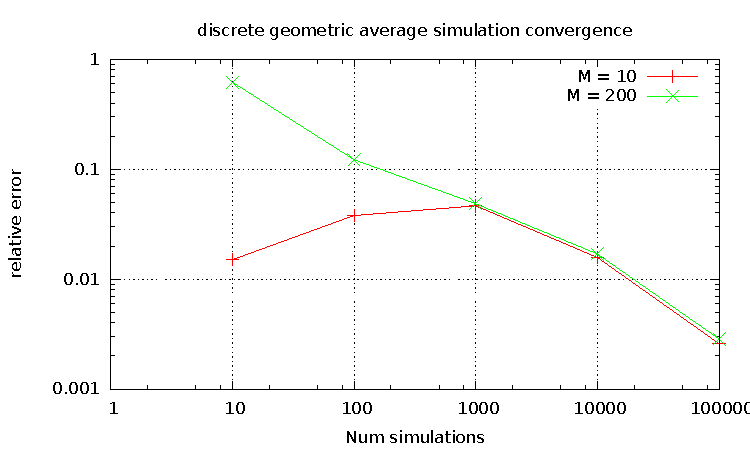
\includepdf{../Task03/sh3_task3_convergence_plot.pdf}
We assume that the convergence should go to zero. This is maybe connected to the fact that our implementation of the closed solution differs from the closed solution is given by the side "http://www.quantcalc.net/DGA.html" but our simulation doesn't converge either way. 
\begin{figure}[htbp]
  \centering
     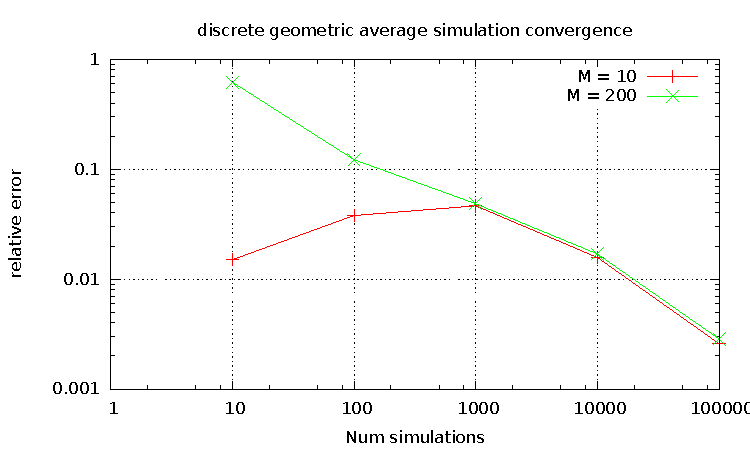
\includegraphics[width=1.0\textwidth]{../Task03/sh3_task3_convergence_plot.pdf}
%    \caption{}
\end{figure}
\newpage
This behavior is not desired. We would expect the error getting smaler, but this is maybe connected to behavior in task 3.
\section*{Task: 4}
\begin{figure}[htbp]
  \centering
     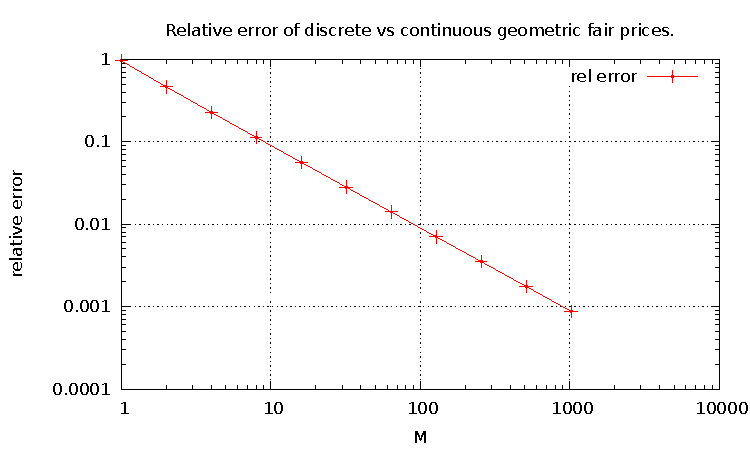
\includegraphics[width=1.0\textwidth]{../Task04/sh3_task4_convergence_plot.pdf}
%    \caption{}
\end{figure}

\section*{Task: 5}

\begin{figure}[htbp]
  \centering
     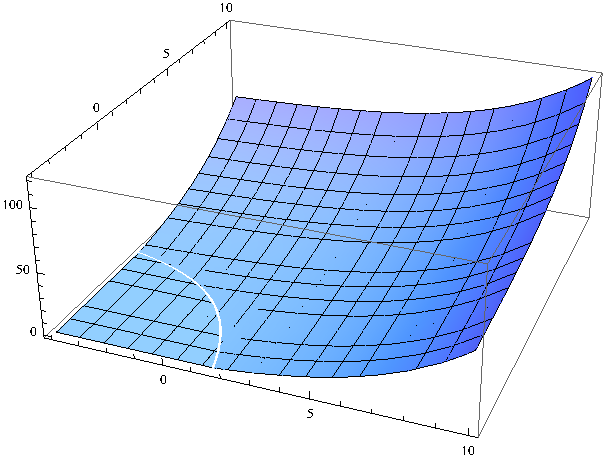
\includegraphics[width=0.8\textwidth]{../Task05/sh3_task5_arithmetic_payoff.pdf}
%    \caption{}
\end{figure}
\newpage
\section*{Task: 7}

\begin{figure}[htbp]
  \centering
     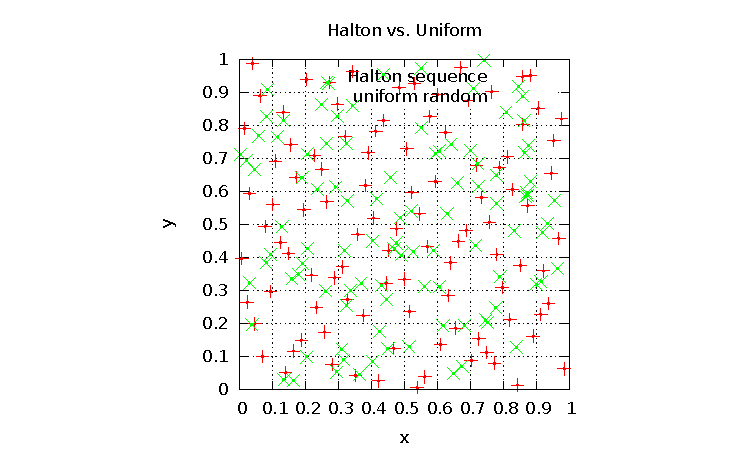
\includegraphics[width=1.0\textwidth]{../Task07/sh3_task7_point_plot.pdf}
%    \caption{}
\end{figure}

\section*{Task: 9}

\begin{figure}[htbp]
  \centering
     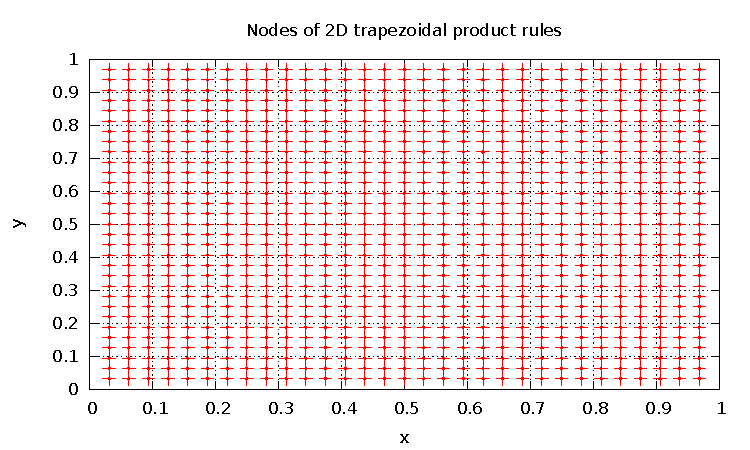
\includegraphics[width=1.0\textwidth]{../Task09/sh3_task9_point_plot_trapezoidal.pdf}
%    \caption{}
\end{figure}
\newpage
\begin{figure}[htbp]
  \centering
     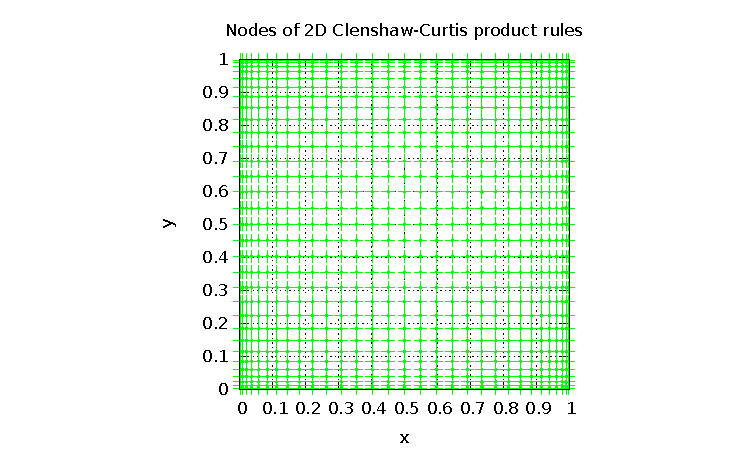
\includegraphics[width=1.0\textwidth]{../Task09/sh3_task9_point_plot_clenshawCurtis.pdf}
%    \caption{}
\end{figure}

\begin{figure}[htbp]
  \centering
     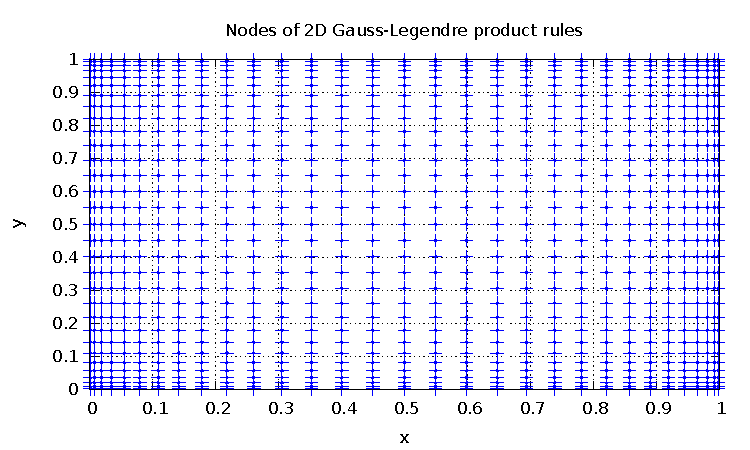
\includegraphics[width=1.0\textwidth]{../Task09/sh3_task9_point_plot_gaussLegendre.pdf}
%    \caption{}
\end{figure}
\newpage
\section*{Task: 11}

\begin{figure}[htbp]
  \centering
     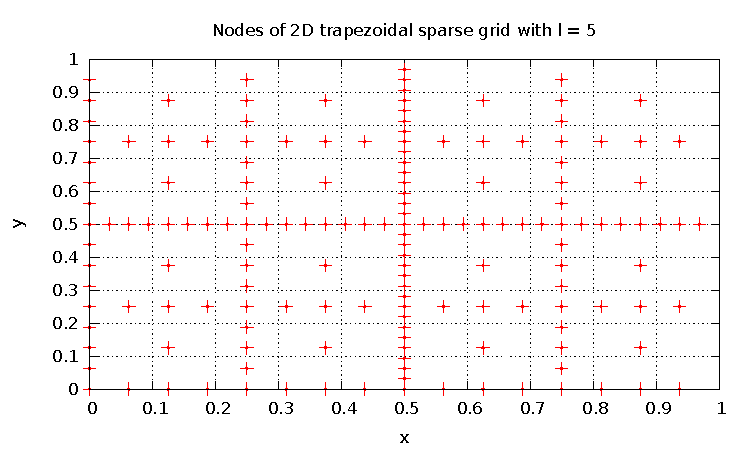
\includegraphics[width=1.0\textwidth]{../Task11/sh3_task11_point_plot_trapezoidal_l=5.pdf}
%    \caption{}
\end{figure}

\begin{figure}[htbp]
  \centering
     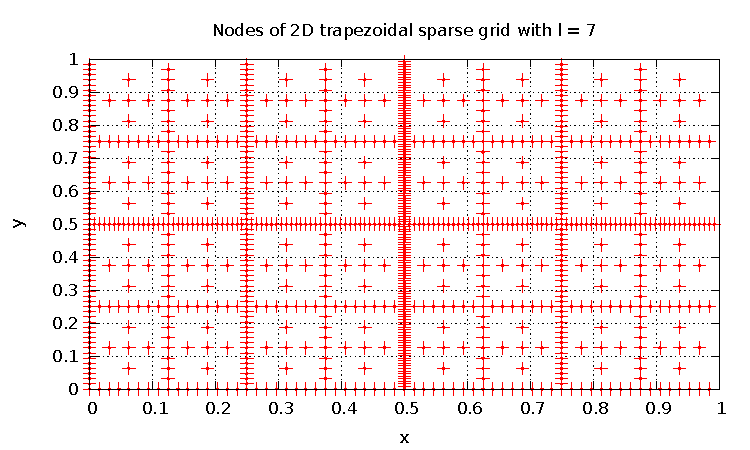
\includegraphics[width=1.0\textwidth]{../Task11/sh3_task11_point_plot_trapezoidal_l=7.pdf}
%    \caption{}
\end{figure}
\newpage
\begin{figure}[htbp]
  \centering
     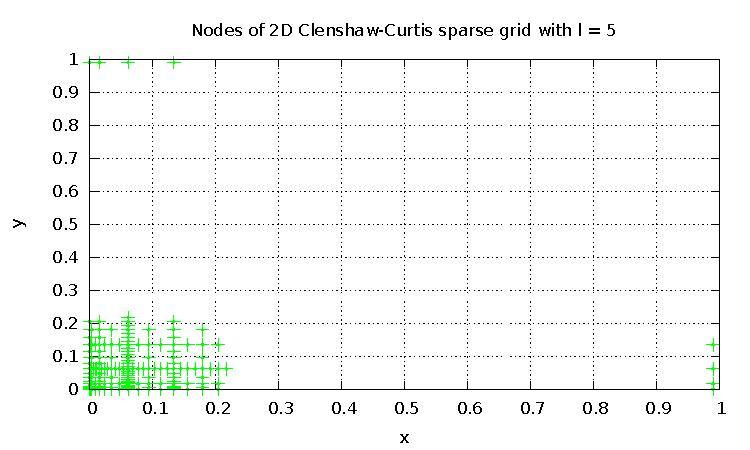
\includegraphics[width=1.0\textwidth]{../Task11/sh3_task11_point_plot_clenshawCurtis_l=5.pdf}
%    \caption{}
\end{figure}

\begin{figure}[htbp]
  \centering
     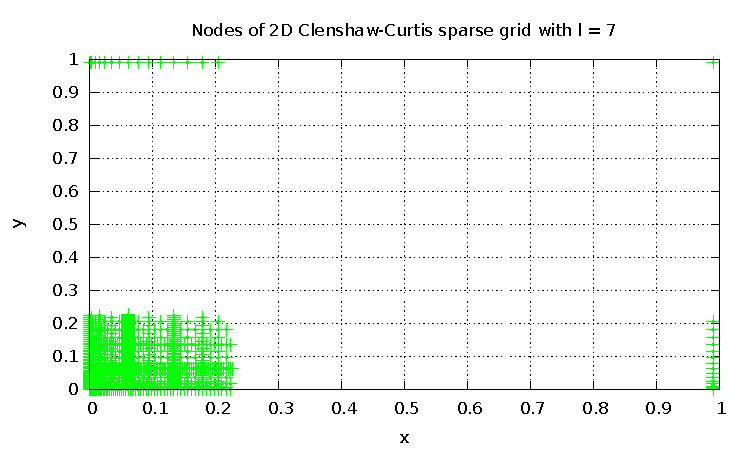
\includegraphics[width=1.0\textwidth]{../Task11/sh3_task11_point_plot_clenshawCurtis_l=7.pdf}
%    \caption{}
\end{figure}
\newpage
\section*{Task: 12}

\begin{figure}[htbp]
  \centering
     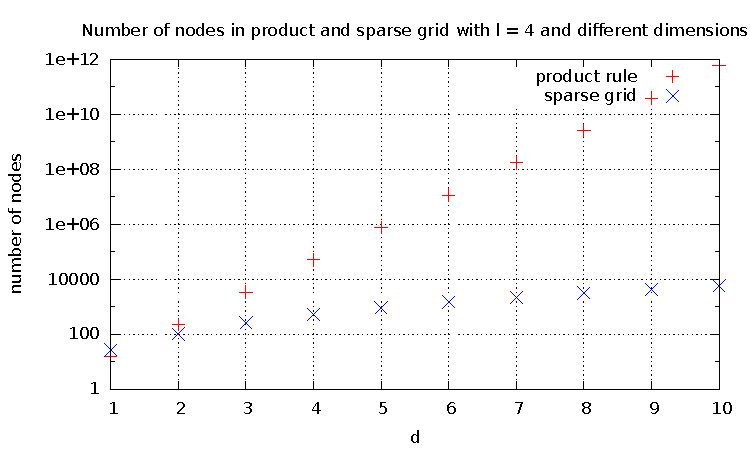
\includegraphics[width=1.0\textwidth]{../Task12/sh3_task12_num_of_nodes.pdf}
%    \caption{}
\end{figure}

\section*{Task: 13}

\begin{figure}[htbp]
  \centering
     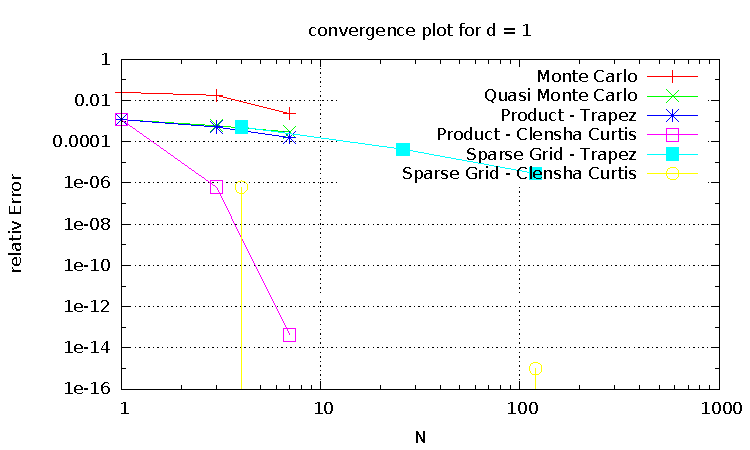
\includegraphics[width=1.0\textwidth]{../Task13/sh3_task13_convergencePlotd1.pdf}
%    \caption{}
\end{figure}
\newpage
\begin{figure}[htbp]
  \centering
     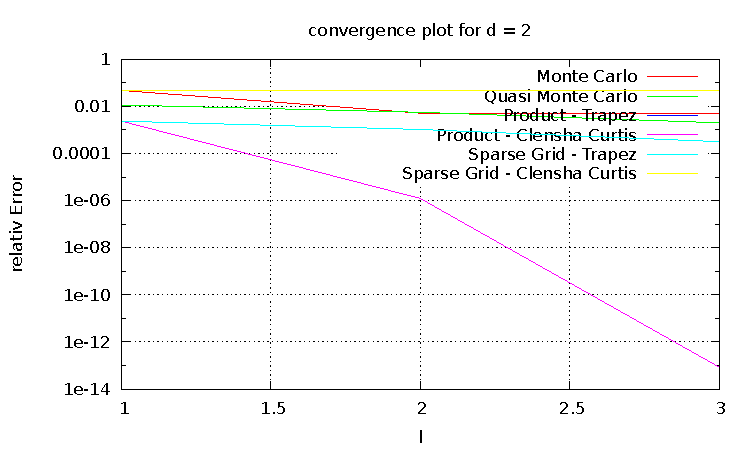
\includegraphics[width=1.0\textwidth]{../Task13/sh3_task13_convergencePlotd2.pdf}
%    \caption{}
\end{figure}

\begin{figure}[htbp]
  \centering
     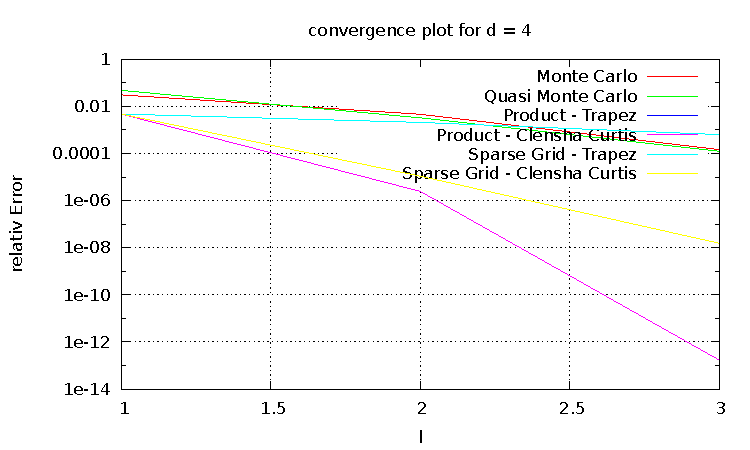
\includegraphics[width=1.0\textwidth]{../Task13/sh3_task13_convergencePlotd4.pdf}
%    \caption{}
\end{figure}
\newpage
\begin{figure}[htbp]
  \centering
     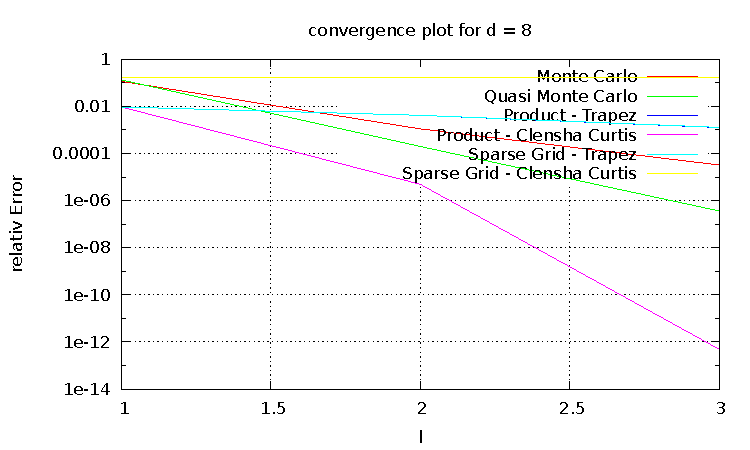
\includegraphics[width=1.0\textwidth]{../Task13/sh3_task13_convergencePlotd8.pdf}
%    \caption{}
\end{figure}

\section*{Task: 15}

With level 4 and the given values the integration of both simulations is 10.4889.
\newpage
\section*{Task: 16}

\begin{figure}[htbp]
  \centering
     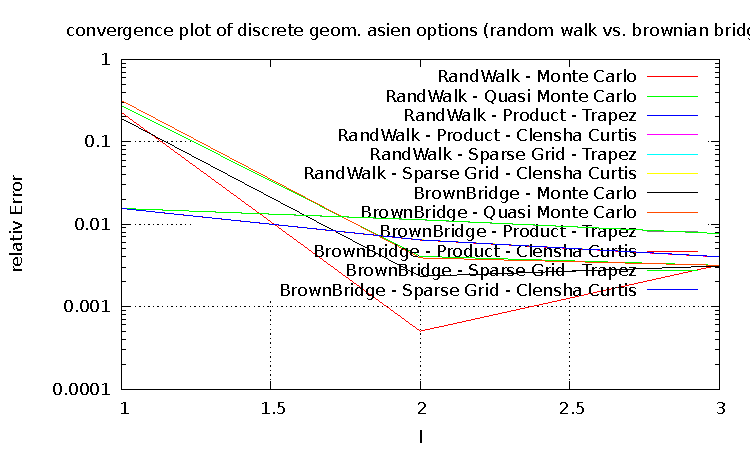
\includegraphics[width=1.0\textwidth]{../Task16/sh3_task16_convergence_plot.pdf}
%    \caption{}
\end{figure}

\section*{Task: 17}
We can't explait this behavior, but we are aware of its wrong nature :)
\begin{figure}[htbp]
  \centering
     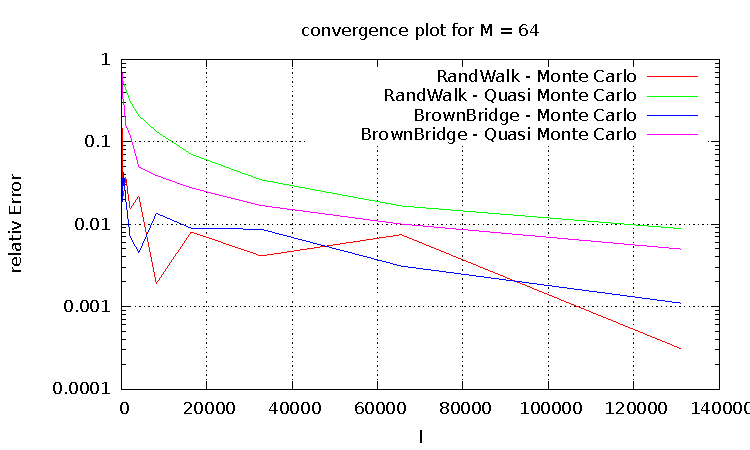
\includegraphics[width=1.0\textwidth]{../Task17/sh3_task17_convergencePlot.pdf}
%    \caption{}
\end{figure}

\newpage

\section*{Task: 18}

Because of the impact of the dimension into the convergence rate, 
the product rule should be used for low dimensions, 
the sparse grid can be used for higher dimensions, then quasi Monte Carlo and
for any high dimension the Monte Carlo integration method whichs convergence rate does not depend on the dimension. 

\end{document}